\section{Boundary conditions}
	A simulation must necessarily have finite extent, we need to employ boundary condtions
	to deal with the edges of the simulation. Here we will go through \(3\) different schemes
	corresponding to periodic boundaries, Dirichlet conditions and Von Neumann conditions.
	Periodic conditions is used when we want to simulate an infinite plasma sheet.
	It is fitting to use when the plasma sheet is of a much larger extent than the
	length scale of the phenomen we want to investigate. (Rewrite sentence)
	Dirichlet conditions is useful when the voltage on the edge of the simulation
	can be known beforehand, as it is often in laboratory experiments (citation?).
	When the electric field, or alternatively gradient of the voltage, along the edges is known
	von Neumann conditions should be used. The boundary conditions must also be coupled
	with fitting boundary conditions applied to the particles in a full PiC simulation.
	Particle conditions include periodic, bouncing and absorbing boundaries.
	To maintain the design aim of inherent modularity of our PiC model, the boundary conditions
	are defined using ghost points, avoiding different discretization stencils at
	the boundary. This reduces the complexity the smoothers, makes the boundary
	conditions easier to implement and opens the possiblity of using them with other
	solvers.


\subsection{Periodic Boundaries}
	With periodic boundary conditions we want the boundary on one side to be equal
	to the field on the other side of the plasma. For the \(1\)D case, see \cref{fig:periodic},
	this can be written as

	\begin{equation}
		\nabla^2 \phi = -\rho \qquad \Omega = [0,L]
	\end{equation}

	With boundaries

	\begin{equation}
		\phi(0) = \phi(L)
	\end{equation}

	Here we should note that this is very similar to what happens between the subdomains
	in a Domain Partitioning parallelization scheme, so often the same algorithm and code
	can be reused to achieve periodic boundary conditions.

	Solutions for the contineous problem with periodic boundary conditions exists only if
	the \textit{compatibility condition} \citep{trottenberg_multigrid_2000}

	\begin{equation}
			\int_\Omega \rho\differential \vb{x} = 0
	\end{equation}

	is held. This means that the total charge in the domain must be zero, which
	is often true in plasma due to quasi-neutrality.


\subsection{Dirichlet Boundaries}
	With Dirichlet conditions the boundaries of the potential are known and given by a function,
	\(\partial\Omega\). Then a \(1\)D problem, \cref{fig:dirichlet} , is represented by

	\begin{equation}
		\nabla^2 \phi = -\rho \qquad \Omega = [0,L]
	\end{equation}
	with boundaries
	\begin{equation}
		\phi(0) = \partial \Omega(0), \qquad \phi(L) =  \partial\Omega(L)
	\end{equation}


\subsection{Neumann Boundaries}
	Now we assume we know the gradient of the potential along the boundary, \(\nabla\phi_{\partial \Omega} = f\).
	This is often used in hydrodynamics to represent reflecting boundaries.
	Then our \(1\)D example problem will look like

	\begin{equation}
		\nabla^2 \phi = -\rho \qquad \Omega = [0,L] \label{eq:1D_poisson}
	\end{equation}
	with boundaries
	\begin{equation}
		\partial \phi(0) = f(0), \qquad \partial \phi(L) = f(L)
	\end{equation}

	The boundary condition is then stated as a gradient and we need to approximate it
	to \(\phi\) to use it in the poisson equation, \cref{eq:1D_poisson}.
	We do this by a \(2\)nd order central difference to the gradient.

	\begin{equation}
		\pdv{\phi(x)}{x} = \frac{\phi(x +\Delta x ) - \phi(x -\Delta x )}{2\Delta x} = f(x)
	\end{equation}

	At the lower boundary, \(x=0\), this can then be written as
	\begin{equation}
		\phi(-\Delta x) = \phi(\Delta x) - 2\Delta x f(0) \label{eq:neumann_lower}
	\end{equation}
	and at the upper
	\begin{equation}
		\phi(L + \Delta x) = \phi(L + \Delta x) - 2\Delta x f(L) \label{eq:neumann_upper}
	\end{equation}

	With our discretization, where the internal cell sizes are \(1\), the \(\phi(-\Delta x)\)
	correspond directly to a ghost cell. So we can implement the Neumann boundary conditions
	easily by setting the ghost cells equal to \cref{eq:neumann_lower,eq:neumann_upper},
	see \cref{fig:neumann}.
	This scheme completely avoids any modification of the smoother stencils at the boundaries.




	%Color scheme
	\tikzstyle{true}=[circle,fill=blue!40,minimum size=25pt,inner sep=0pt]
	\tikzstyle{ghost}=[circle,fill=black!40,minimum size=25pt,inner sep=0pt]
	\tikzstyle{changed} = [circle,fill=red!40,minimum size=25pt,inner sep=0pt]


	\begin{figure}
		\centering
		\begin{subfigure}[b]{0.9\textwidth}
			\centering
			
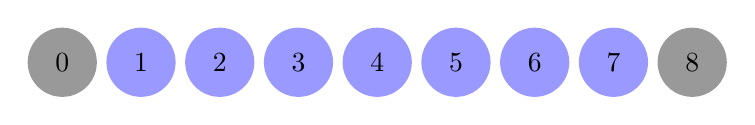
\begin{tikzpicture}%[scale=1, auto,swap]
    %True nodes
    \foreach \pos/\name in 	{{(1,0)/1}, 	{(2,0)/2},	{(3,0)/3},
                             {(4,0)/4},	{(5,0)/5}, {(6,0)/6}, {(7,0)/7}}
    \node[true] (\name) at \pos {$\name$};
    %Ghost nodes
    \node[ghost] (0) at (0,0) {$0$};
    \node[ghost] (8) at (8,0) {$8$};
\end{tikzpicture}

			\caption{A \(1\) dimensional domain with grid points before the boundary conditions has been applied.
			The numbers denote the indexes for the values in the grid array. The blue grid points, (\si{1\to 7}) represents
			the true grid and the grey points, (\si{0,8}), is the ghost cell values. The consepts shown here should easily be
			expanded to more dimensions.}
			\label{fig:initial}
			% \caption{}
		\end{subfigure}
		\begin{subfigure}[b]{0.9\textwidth}
			\centering
			\input{tikz/periodic}
			\caption{Here periodic boundary conditions has been applied to the \(1\)D domain above. Here and in the following the
			red color means a point has been changed. The ghost points at the edges has been set to equal the
			true grid points at the opposite edge giving periodic boundary conditions.}
			% \caption{}
			\label{fig:periodic}
		\end{subfigure}
		\begin{subfigure}[b]{0.9\textwidth}
			\centering
			
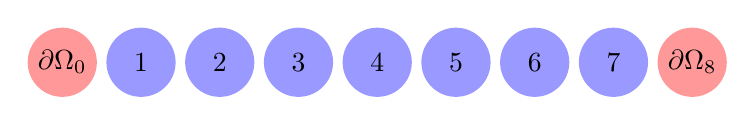
\begin{tikzpicture}%[scale=1, auto,swap]
    %True nodes
    \foreach \pos/\name in 	{{(1,0)/1}, 	{(2,0)/2},	{(3,0)/3},
                             {(4,0)/4},	{(5,0)/5}, {(6,0)/6}, {(7,0)/7}}
    \node[true] (\name) at \pos {$\name$};
    %Ghost nodes
    \node[changed] (0) at (0,0) {$\partial\Omega_0$};
    \node[changed] (8) at (8,0) {$\partial\Omega_8$};
\end{tikzpicture}

			\caption{For Dirichlet boundary conditions we have predetermined values along the edge, this are here represented as the ghost cells
			being set to a given value defined by \(\partial\Omega_i\). The boundary function can be as simple as setting everything along
			the edge to a constant, but it could also be a spatially and time varying function. It is also possible to let it correspond to
			input given by coupled computer model.}
			% \caption{}
			\label{fig:dirichlet}
		\end{subfigure}
		\begin{subfigure}[b]{0.9\textwidth}
			\centering
			\input{tikz/neumann}
			\caption{Von Neumann boundary conditions specifies what the derivative is on the edge. To achieve that we set the ghost points to
			a specified value that will give the wanted derivative when a finite difference method swipes over the point. For the left side
			the function should be set to \(f_0 = u_2 - 2\Delta x A\) and to \(f_8 = u_6 - 2\Delta x A\) for the right side. Here \(A\) is the
			predetermined values that the derivative should correspond to.}
			% \caption{}
			\label{fig:neumann}
		\end{subfigure}
		\caption{An overview of 3 boundary conditions applied to a \(1\)D domain.}
	\end{figure}
